\documentclass[11pt]{article}
%\setlength{\headheight}{13.59999pt}
\usepackage[utf8]{inputenc}

\title{Luminosity function}
\author{Henrik Andrews}
\usepackage[backend=biber,style=authoryear]{biblatex}
\addbibresource{bibfile.bib}

\usepackage{hyperref}





\usepackage{subcaption}
\usepackage[ portrait, margin=2.54cm]{geometry}
\usepackage{graphicx}
\usepackage{amsmath}
\usepackage{setspace}
\usepackage{upgreek}
\usepackage{bbold}
\usepackage{fancyhdr}
\usepackage{mathtools}
\usepackage{tabularx}
\usepackage{lipsum}
\usepackage[dvipsnames]{xcolor}
\usepackage{pdfpages}
\setlength{\parindent}{0em}
\setlength{\parskip}{1em}
\usepackage{caption}
\usepackage{multicol}	
\usepackage[most]{tcolorbox}


\usepackage{float}
\newcommand{\HRule}[1]{\rule{\linewidth}{#1}}
\usepackage{listings}
\usepackage{color} %red, green, blue, yellow, cyan, magenta, black, white
\definecolor{mygreen}{RGB}{28,172,0} % color values Red, Green, Blue
\definecolor{mylilas}{RGB}{170,55,241}
\definecolor{backcolour}{rgb}{0.95,0.95,0.92}

\newtcolorbox{mycomment}[2][]{
  colback=red!5!white,
  colframe=red!55!black,
  fonttitle=\bfseries,
  title=#2,
  #1
}

\setstretch{1.25} %line spacing

\begin{document}

\title{ \normalsize
	\HRule{0.5pt} \\
	\LARGE \textbf{{Luminosity functions of Active galactic nuclei and their emissivity of UHECRs and neutrinos}}	
	\\
	\HRule{2pt} \\ [0.5cm]		
%fix the university logo !!!!!!!!!!!!!!!!!!!!!!!!
	\vspace{6cm}
	\begin{figure}[htp]
    \centering
    
\includegraphics[width=.2\textwidth]{Logo-Ntnu.svg.png}
    \end{figure}
	}

\author{
    \normalsize 
	\textbf{Henrik Døvle Andrews } \\
	Norwegian university of Science and Technology \\ 
}

\maketitle
\setcounter{page}{ 0 }

\newpage

\pagestyle{fancy}
\fancyhf{}
\setlength\headheight{14pt}
\fancyhead[L]{Henrik Døvle Andrews}
\fancyhead[R]{\leftmark}
\fancyfoot[R]{Page \thepage \:}
\setcounter{page}{1}


\maketitle


\section{Compact symmetric objects(CSO)}

Compact symmetric objects represents a class of compact (< 1kpc) bright double radio sources, where the radio lobes straddle the AGN.
They are further separated into two classes CSO 1 and 2, where 1 are less luminous and CSO 2 which will be the focus are edge-brightened high Luminosity class. 
CSO 2 separate themselves from FR1 and FR2 in their size, but also in their lifespan. In \cite{sullivan2024smallscale} they suggest that CSO 2s have a short lifespan $<10^4$ years.
Furthermore, CSO 2 are divided into three sub categories based on where in their life cycle they are, these are: CSO 2.0, 2.1 and 2.2. 

CSO 2 distinguish themselves from other jetted AGNs in lobe morphology, size, and reletivistic beaming towards the observer. 

Their CSO catalog has 79 bone fide CSO2s, 54 of which have spectroscopic redshifts measured. 

There is a distinct cutoff in numbers of CSO 2 when moving to bigger sizes suggesting a discountinuity between CSO 2 and larger symmetric objects, also questioning the postulation that CSOs are the early versions of larger FR objects. 
a max of $5\%$ should evolve into larger objects. 



\subsection{jet model}
The model of the jet evolution and structure is similar to FR II soruces, and in \cite{Bromberg_2011} they go throught a model of an unmagnetized and gas pressured collumated jet model.  
the heigth of the jet has a speed that is propotional to \begin{mycomment} {} I find it strange that they use a model for a collimated jet when we are talking about a different morphology\end{mycomment}

\begin{equation}
    v_h \simeq \sqrt{\frac{L_j}{\rho_a A_j c}}
\end{equation}
here $L_j$ is the jet power, $\rho_a$ is the ambient density of the external medium, $A_j$ is the jet cross section and c is the speed of light

The height of the shock follows the mach cone as 

\begin{equation}
    \zeta = \sqrt{\frac{L_j}{P_c\pi c}}
\end{equation}

The pressure in the cocoon is then given by
\begin{equation}
    P_c = \frac{1}{3}\frac{E(t)}{\pi r_c^2\zeta} = \frac{1}{3}u_{int}
\end{equation}


With the cocoon pressure equaling the ram pressure on gets

\begin{equation}
    v_c = \sqrt{\frac{P_c}{\rho_a}}
\end{equation}





\subsection{First tests }
from \cite{bronzini2024investigating} they found the x-ray Luminosity to be between $10^{41}$ and $10^{45}$ erg/s.
From figure 11 in \cite{readhead2023compact} one sees that the average expected luminosity is approximatly $2*10^{43}$ erg/s.

\begin{itemize}
    \item from \cite{readhead2023compact} space density of CSO 2 is $1.2 * 10^4 $Gpc3 = $1.2 * 10^{-5} Mpc^3$
    \item from \cite{readhead2023compact} the average luminosity is $2*10^{43}$ erg/s
    \item same source gives that the size of CSOs 2.0 is $0.126$ kpc and CSO 2.2 is $0.3$ kpc
    \item \cite{bronzini2024investigating} finds that the magnetic field is $10^{-2}$ G based on the equipartition argument. This is in the lobes of the jet. But these will engulf the AGN due to the nature of CSOs 
\end{itemize}
NB! most of these measurments I believe are based on the total class of CSO, not only CSO 2. CSO 2 is the brightest of the CSO classes, where the jet has not stalled, \cite{readhead2023compact}

\begin{figure}
    \centering
    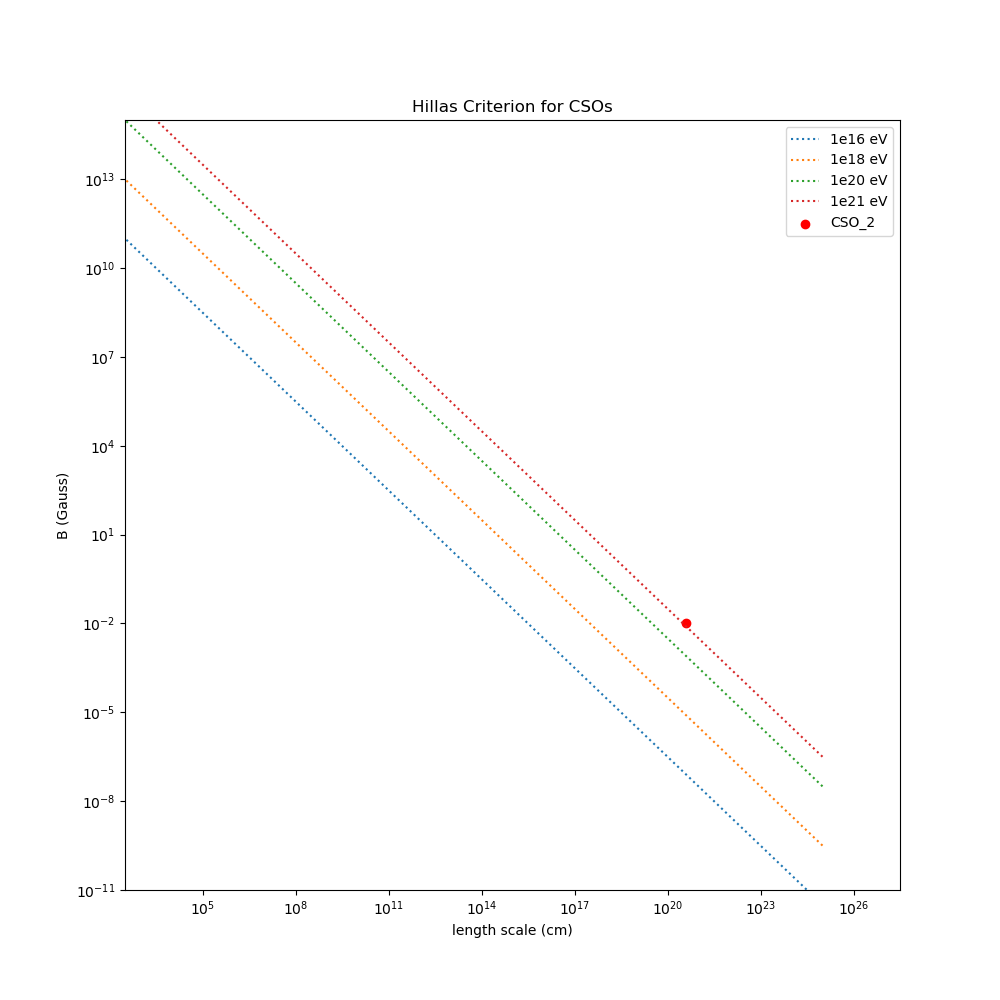
\includegraphics[width=0.7\textwidth]{Plots/Hillas_criterion_CSO.png}
    \caption{Hillas criterion for all CSO}
    \label{fig:Hillas_criterion_CSO}
\end{figure}


\begin{figure}
    \centering
    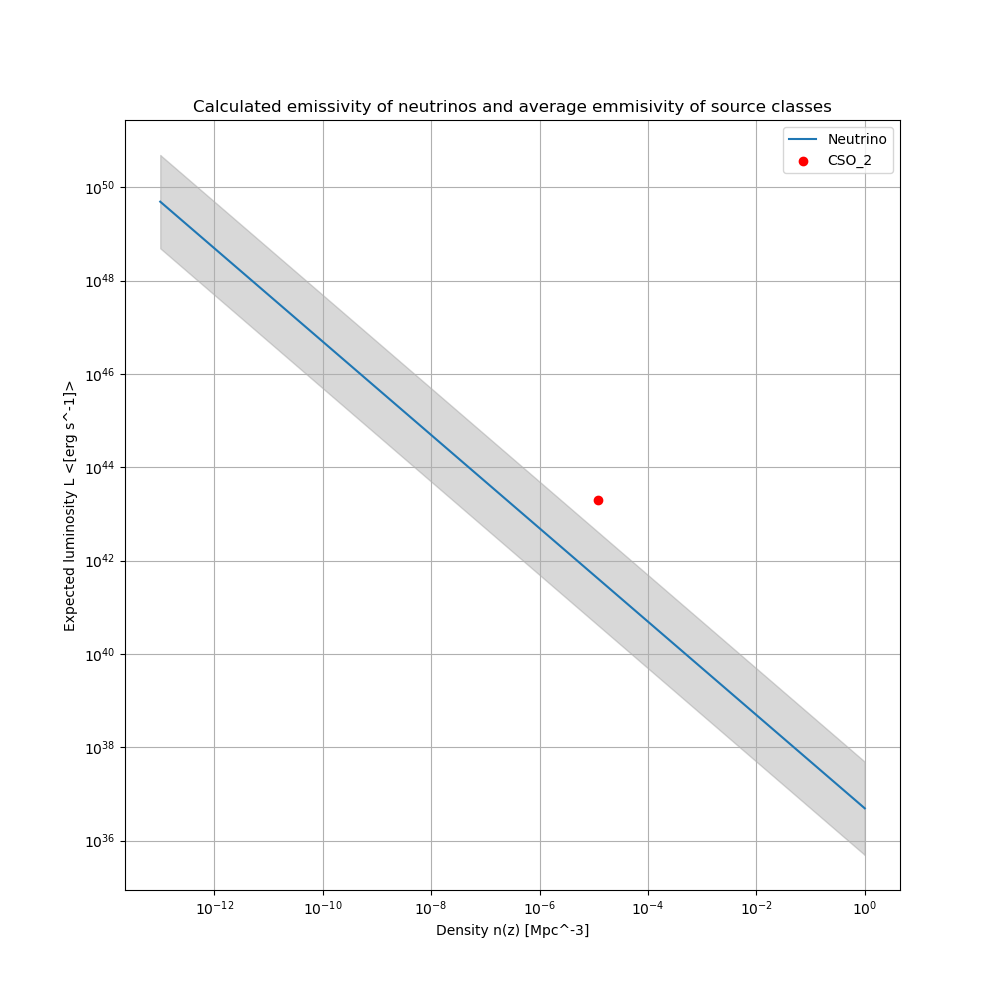
\includegraphics[width=0.7\textwidth]{Plots/L_n_neut_calc_cso.png}
\end{figure}

\begin{figure}
    \centering
    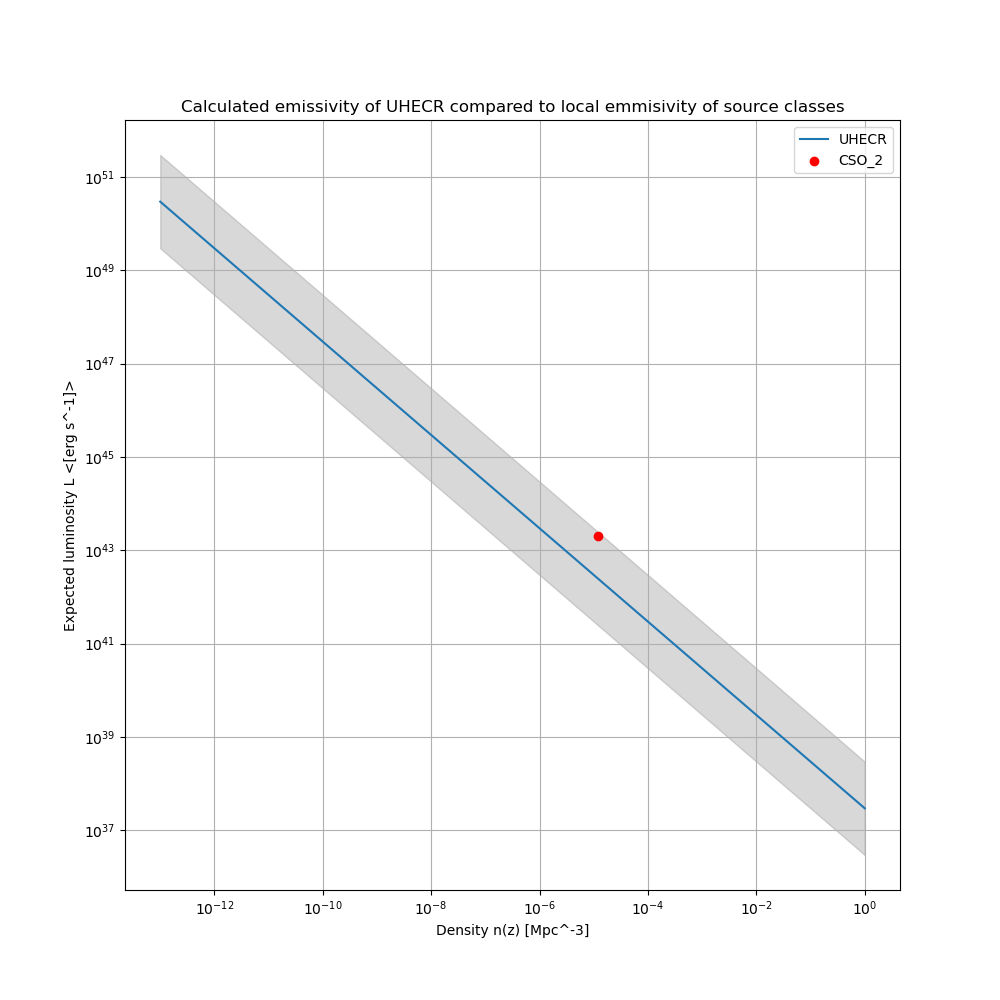
\includegraphics[width=0.7\textwidth]{Plots/L_n_uhecr_calc_cso.png}

\end{figure}



\subsection*{Kinetic Jet power in CSO 2 against UFO}
In \cite{bronzini2024investigating} he discusses two CSOs which are located quite close to earth, and which have had 
quite a bit of research done on them. These are PKS 1718-649 in galaxy NGC 6328 and TXS 1146+596  in galaxy NGC 3894. Only TCXS 1146+596 has enough of a broad band spectrum to
estimate both the accretion rate and minimum kinetic jet power. This is done in \cite{Balasubramaniam_2021} and the value for both is 
\begin{equation}
    L_{kin} = 2 * 10^{42} erg/s,
\end{equation}
and 

\begin{equation}
    \lambda_{Edd} = \frac{L_{bol}}{L_{Edd}} \approx 10^{-4}.
\end{equation}

This is for one source, but it will serve as a benchmark for other CSOs of its type. Of course, it is not optimal 
to assume that all CSOs have the same kinetic power, but if one adds more requirements it could work. The biggest supplementary 
requirement could be kinematic age, which is the time it takes for the jet to reach the size it is at. 

To compare this one will look at the kinetic power of UFOs, which are studied in \cite{peretti2023diffusive}. In it they find that the kinetic power of UFOs is
proportional to the bolometric luminosity of the AGN. They actually cite \cite{Fiore_2017} who gives the relation between mass outflow rate and bolometric luminosity. 
In \cite{peretti2023diffusive} they then argue that the kinetic power of the UFOs is approximately $3$ percent of the bolometric luminosity. 

\begin{figure}
    \centering
    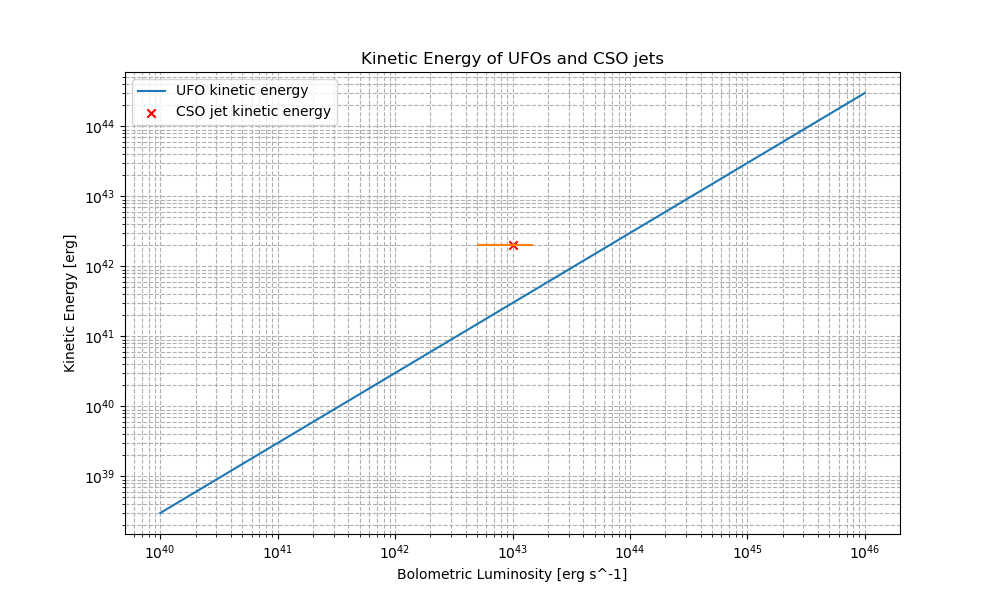
\includegraphics[width=0.7\textwidth]{Plots/Kinetic_energy_UFO_CSO.png}
    \caption{Kinetic power of CSO 2}
    \label{fig:L_kin_cso}
\end{figure}
Here we see the comparison with the kinetic power of UFOs. The UFOs are a bit less powerful than the CSO 2s, but not by much.

\section*{Timescales}
\subsection*{Dynamical time}
The variablility time scale will set the dynamical timescale of our system. in order to find it one must 
analyse the SED of different sources. Usually one take the x-ray variablility since it is closly related to the 
accretion disk. If no variablility is found one can then instead use the size of the system, but variablility would confine the acceleration region better. 

from \cite{bronzini2024investigating} which did the SED of two CSOs they found no variablility over the timescales of years in 1146+596 and for 1718-649 they found a variablility of a factor of 2.5 on the timescales of years. The source where this timescale is 
taken from also ambigouisly states that the variablility is in years, \cite{Beuchert_2018}. 

One does not need to use only one size of the system, but look at what different sizes would say. From 
\cite{bronzini2024investigating} one has the emmiting region of two different models and also the lobes. One can include this to see what the differences are. 




\newpage
\printbibliography
\end{document}